\documentclass[a4paper,11pt]{article}
% \usepackage[british,UKenglish]{babel}
% \usepackage[version=3]{mhchem}
% \usepackage{bm}
% \usepackage{multirow}
% \usepackage{mathtools}
\usepackage{graphicx}
\usepackage{framed}
\newcommand{\bs}{\boldsymbol}
% \newcommand{\mr}{\mathrm}
\usepackage{parskip} %per avere spaziatura verticale tra paragrafi e non indentazione
\usepackage{enumitem}
\usepackage{fullpage}
\usepackage{amsmath}
\bibliographystyle{jphysicsB}
% \usepackage{sfmath}
\renewcommand{\familydefault}{\sfdefault}
\makeatletter
\newcommand\footnoteref[1]{\protected@xdef\@thefnmark{\ref{#1}}\@footnotemark}
\makeatother

% Documentation for commands
\newcommand{\cmddoc}[1]{\vskip10pt
\texttt{#1}}
% 

\begin{document}

\Large
\begin{center}
\textbf{EXAT \\ Excitonic Analysis Tool}
\end{center}
\normalsize
\begin{center}
\emph{Sandro Jurinovich}\footnote{\texttt{sandro.jurinovich@for.unipi.it}},
\emph{Lorenzo Cupellini}\footnote{\texttt{lorenzo.cupellini@for.unipi.it}},
 Ciro Guido \& Benedetta Mennucci
\end{center}

\section{Version}

This documentation refers to version 1.0.0 

Although the development is devoted to mantain the compatibility with previous versions, the newer versions will probably show small differences in the behaviour of the program or in the defaults, in addition to new features. Before using the program, check that the version corresponds to the one reported in this manual.

\section{Presentation}

\texttt{EXAT} (Excitonic Analysis Tool) is a Molecolab tool\footnote{\texttt{http://molecolab.dcci.unipi.it} ---
For help or to require a copy of the program, please write to
\texttt{benedetta.mennucci@unipi.it}.}. 


The program performs excitonic calculations from external input, or from the results of Gaussian (R) 16 calculations.

\begin{figure*}[!hb]
 \centering
 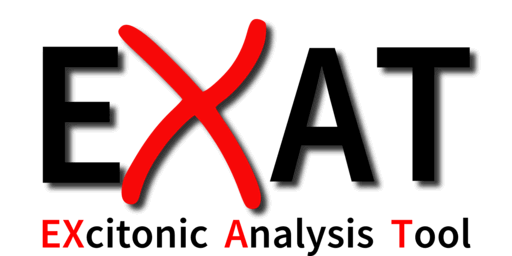
\includegraphics[width=0.5\textwidth]{logo.png}
\end{figure*}


\section{Usage}

\subsection{Software prerequisites and compiling}

\texttt{EXAT} is written in Python. The \texttt{numpy} and \texttt{scipy} packages are needed. Additionally, \texttt{matplotlib} is needed to view the excitonic spectrum.  


\subsection{Needed input files}\label{sec:input}

Before running EXAT, you need a calculation with Gaussian16 on the system of interest with the \texttt{eet=fragment} keyword. An example input file is shown in the following
\begin{quote}
\begin{verbatim}
#p td(nstates=4) b3lyp/6-31G(d) eet(fragment=4)

Title line

0 1 
[geometry]

\end{verbatim}
\end{quote}

\textbf{Important:} note that the \texttt{\#p} keyword specified in the route section generates additional print that \texttt{EXAT} will read, and therefore is needed to perform the excitonic calculation.

Alternatively, you can provide external files with site energies, couplings, and dipole moments (see below).

The optional \texttt{chromlist} file should be specified in order to use the \texttt{--seltran} option (see the Usage). The file shoud contain the selected chromophores, one per line. The first column contains the chromophore number; the transitions to select should be specified on the same line Here is an example of a \texttt{chromlist.in} file:

\begin{quote}
\begin{verbatim}
1  1 2
3  1 2 4
4  1 3
\end{verbatim}
\end{quote}

This input tells \texttt{EXAT} to consider only fragments \texttt{1}, \texttt{3}, and \texttt{4}, and to select transitions 1 and 2 of chromophore 1, transitions 1, 2 and 4 of chromophore 3, and transitions 1 and 3 of chromophore 4.


\subsubsection{External input}\label{sec:input_ext}

\texttt{EXAT} is able to read input from external text files. In this case, several input files are needed. A \texttt{chromlist} file as described in Section~\ref{sec:input} is required, and the transitions should always be specified. The total number of transitions is calculated from the transitions specified in this file.

\paragraph*{Site energy file. } 
This file specifies the energy of the transitions. Its default name is \texttt{site.in}. It should specify the transition energy of every chromophore, one line per chromophore, \emph{in the same order as the \texttt{\emph{chromlist}} file.} The first column should contain the chromophore number. The other column should contain the site energies of the transitions. For example:

\begin{quote}
\begin{verbatim}
1  1.56 2.20
3  1.58 2.14 2.60
4  1.60 2.60
\end{verbatim}
\end{quote}

\paragraph*{Dipoles file. } 
This file specifies the transition dipole moments. Its default name is \texttt{dipo.in}. It should contain a line for every transition, specifying the components $x$, $y$ and $z$ of the transition dipole. The dipoles should be specified in the same order as in the \texttt{chromlist} file, and then in the order of the transitions. The dipole moment units are Debye.

\paragraph*{Centers file. } 
This file specifies the centers of the transitions. Its default name is \texttt{cent.in}. The format is the same as the dipoles file. The units are Angstrom.

\paragraph*{Coupling file. } 
This file specifies all couplings between transitions on different chromophores. The default name is \texttt{coup.in}. The file contains one coupling per line and should be sorted in increasing order of chromophore and transition (Chrom1 Chrom2 Tran1 Tran2). 

\emph{The format of this file will be changed in later versions.}

\subsection{Running the program}

The command-line call to \texttt{EXAT} depends on the type of input (see Section~\ref{sec:input}). In the next sections the required commands for the various input types are presented.

\subsubsection{Running from Gaussian 16 output}

The command-line syntax for running EXAT from a the Gaussian logfile is:

\begin{framed}
\begin{quote}
\begin{verbatim}
$> exat.py [options] [chromlist] -i logfile
\end{verbatim}
\end{quote}
\end{framed}

where \texttt{logfile} is the Gaussian log file of the EET calculation, and ChromList is the list of fragment as described in Section~\ref{sec:input}. 


\subsubsection{Running with external input}

The text files needed for external input are described in Section~\ref{sec:input_ext}, with their format. The program should be called as:

\begin{framed}
\begin{quote}
\begin{verbatim}
$> exat.py -e [chromlist] [--indipo dipofile] \
  [--incoup coupfile] [--insite sitefile] [--incent centfile]
\end{verbatim}
\end{quote}
\end{framed}

where \texttt{dipofile} contains the transition dipoles, \texttt{coupfile} contains the couplings, \texttt{sitefile} contains the site energies, and \texttt{centfile} contains the transition centers. These files need to be specified only if their name is different from the default name (See Section~\ref{sec:input_ext}).


\subsubsection{Command-line options}

This section describes all command-line options for \texttt{EXAT}. 

\paragraph*{General options:}
\begin{description}[labelsep=10pt, align=left, labelwidth=80pt,labelindent=0pt,leftmargin=90pt]
\item[\texttt{-h}] Show the help message for the command-line options
\item[\texttt{-v}] Increase verbosity of the output. Some files are only printed with high verbosity level.
\item[\texttt{-q}] Quiet output: minimum printout 
\item[\texttt{-V}] Show the program's full version, and exit
\end{description}

\paragraph*{Input options:}
\begin{description}[labelsep=10pt, align=left, labelwidth=80pt,labelindent=0pt,leftmargin=90pt]
\item[\texttt{-e}] Read all input from external files (Sec.~\ref{sec:input_ext}) 
\item[\texttt{-{}-log,-i}] Name of the Gaussian logfile. This option is only valid if \texttt{gdvh36} or \texttt{oldh36} versions are used.
\end{description}

\paragraph*{Output options:}
\begin{description}[labelsep=10pt, align=left, labelwidth=80pt,labelindent=0pt,leftmargin=90pt]
\item[\texttt{-{}-out,-o}] Followed by the prefix for output files 
\item[\texttt{-{}-savecoeff}] Save full precision excitonic coefficients in a \texttt{numpy} file for later use.
\item[\texttt{-{}-savetprod}] Save matrix of triple products for rotatory strength: $\mathbf{R}_{ij}\cdot(\bs{\mu}_i\times\bs{\mu}_j)$
\item[\texttt{-{}-prtcoup}] Followed by a threshold. With the \texttt{-vv} option, the couplings larger than the threshold will be printed. 
\end{description}


\paragraph*{Option for modifying transitions:}
\begin{description}[labelsep=10pt, align=left, labelwidth=80pt,labelindent=0pt,leftmargin=90pt]
\item[\texttt{-{}-seltran}] Activate selection of transitions on the basis of the \texttt{chromlist} file (See Section~\ref{sec:input}). In this case \texttt{chromlist} should contain for each chromophore the transitions to be considered. 
\item[\texttt{-{}-scaletran}] Followed by a file that defines the scaling factor for every transition. Its format is the same as the site energy file  described in Section~\ref{sec:input_ext}. This scales the transition dipoles and couplings consistently.
\end{description}

\paragraph*{Options for site energies:}
\begin{description}[labelsep=10pt, align=left, labelwidth=90pt,labelindent=0pt,leftmargin=100pt]
\item[\texttt{-{}-insite,-{}-site}] Followed by a site energy file. The format of the input file is described in Section~\ref{sec:input_ext}. The site energies read in input will be overridden if a different value is specified.
\end{description}

\paragraph*{Options for Centers:}
\begin{description}[labelsep=10pt, align=left, labelwidth=80pt,labelindent=0pt,leftmargin=90pt]
\item[\texttt{-{}-cent}] Followed by a string that specifies how to compute the chromophore center. The \texttt{geom} option tells \texttt{EXAT} to compute the center as the geometrical center of the chromophore, while \texttt{mass} is used to compute the chromophore center as the center of mass of the chromophore.Finally, a range of atoms can be specified as a string; the center will be computed as the geometrical center of these atoms. 
\item[\texttt{-{}-incent}] Followed by a center file. The format of the center file is described in Section~\ref{sec:input_ext}. The calculated centers will be overridden.
\end{description}

\paragraph*{Options for Couplings:}
\begin{description}[labelsep=10pt, align=left, labelwidth=80pt,labelindent=0pt,leftmargin=90pt]
\item[\texttt{-{}-coup}] Followed by the coupling calculation type. This option cannot be used with external input. The \texttt{trden} option includes all terms in the coupling. Option \texttt{coulomb} includes only the Coulomb term of the coupling. Option \texttt{PDA} turns off the coupling reading from Gaussian files and computes couplings with the point-dipole approximation. The default is \texttt{trden}.
\item[\texttt{-{}-cleancoup}] Followed by a threshold. All couplings below the threshold will be set to zero.
\item[\texttt{-{}-refrind}] Followed by the medium refraction index for point-dipole coupling calculations. This option is only valid with the \texttt{-{}-coup PDA} option.
\item[\texttt{-{}-scalecoup}] Followed by a scaling factor. All couplings will be scaled by that factor. 
\item[\texttt{-{}-incoup}] Followed by a file containing all couplings. The format of the coupling file is described in Section~\ref{sec:input_ext}. Any couplings read from other input will be overridden.
\end{description}

\paragraph*{Options for Transition Dipoles:}
\begin{description}[labelsep=10pt, align=left, labelwidth=80pt,labelindent=0pt,leftmargin=90pt]
\item[\texttt{-{}-scaledipo}] Followed by a scaling factor. All transition dipoles will be scaled by that factor.  
\item[\texttt{-{}-reorient}] Followed by the IDs of two atoms that define an axis, with respect to which the transition dipoles will be reoriented. Signs of transition dipoles will be changed until all dipoles point in the same direction as the defined axis. The signs of the couplings will be changed accordingly.
\item[\texttt{-{}-forcedipo}] If used with the \texttt{-{}-reorient} option, forces the dipole to be parallel to the defined axis.
\item[\texttt{-{}-anadipo}] Followed by an input file that specifies a reference frame for every chromophore defined in \texttt{chromlist}. This option activates the transition dipole direction analysis, see Section~\ref{sec:anadipo} for a brief description. It cannot be used with external input.
\item[\texttt{-{}-incent}] Followed by a transition dipole file. The format of the dipole file is described in Section~\ref{sec:input_ext}. The transition dipoles read in input will be overridden.
\end{description}

\paragraph*{Options to compute rotatory strength:}
\begin{description}[labelsep=10pt, align=left, labelwidth=80pt,labelindent=0pt,leftmargin=90pt]
\item[\texttt{-{}-mu}]  Use approximate treatment (electric dipoles only). This is the default.
\item[\texttt{-{}-mag}] Use full treatment (electric and magnetic dipoles) in the gauge-invariant velocity formulation. This option is not compatible with reading from external input.
\item[\texttt{-{}-length}] Use full treatment (electric and magnetic dipoles) in the length formulation. This option is not compatible with reading from external input. 
\end{description}

\paragraph*{Advanced and expert options:}
\begin{description}[labelsep=10pt, align=left, labelwidth=80pt,labelindent=0pt,leftmargin=90pt]
\item[\texttt{-{}-ldaxis}] Followed by the definition of the orientation axis for LD. The LD axis can be \texttt{x}, \texttt{y}, \texttt{z}, or the components separated by a comma. Default is \texttt{z}.  
\end{description}

\section{Output files}

The program prints various files during its execution. The prefix for output files can be choosen with the \texttt{-o} option. Some files are always printed, whereas others are only printed with high verbosity or with specific options.

\paragraph*{Main output files}
\begin{description}[labelsep=10pt, align=left, labelwidth=85pt,labelindent=0pt,leftmargin=95pt]
\item[\texttt{matrix.dat}] The excitonic Hamiltonian (all values in cm$^{-1}$)
\item[\texttt{diag.dat}] Excitonic states, energies and coefficients. The second part of the file contains the squared coefficients
\item[\texttt{results.out}] Excitonic states, squared excitonic dipoles, LD intensity, and rotatory strengths. This file is the input to \texttt{spectrum.py}
\end{description}

\paragraph*{Other default output files}
\begin{description}[labelsep=10pt, align=left, labelwidth=85pt,labelindent=0pt,leftmargin=95pt]
\item[\texttt{geometry.xyz}] The geometry of the considered chromophores. It can be used with VMD to visualize transition dipoles (See below). This is not printed when external input is used.
\item[\texttt{visudipo.vmd}] VMD script to visualize transition dipoles (with the \texttt{vmd -e} command). By default, only the electric dipole of the first transition is visualized. The others can be uncommented directly from the script. 
\item[\texttt{dipo.out}] Transition dipoles of the chromophores, in Debye. This file can be used as external input with the \texttt{-{}-readexternal} option.
\item[\texttt{magdipo.out}] Magnetic transition dipoles of the chromophores.
\end{description}

\paragraph*{Optional output files}
\begin{description}[labelsep=10pt, align=left, labelwidth=85pt,labelindent=0pt,leftmargin=95pt]
\item[\texttt{component.out}] This file is printed when using the \texttt{-{}-mag} option. It contains the various components of the rotatory strength (Approximate, Intrinsic, Extrinsic, Total).
\item[\texttt{site.out}] Site energies of the chromophores, in eV. This file can be used as external input with the \texttt{-{}-readexternal} option.
\item[\texttt{coup.out}] Excitonic couplings larger than the threshold (Specified by the \texttt{-{}-prtcoup} option). The first four columns specify chromophore and transition indices, the fifth column is the coupling, the sixth colum is the distance.
\end{description}


\section{Advanced functions}

\subsection{Dipole analysis}\label{sec:anadipo}

The \texttt{-{}-anadipo} option activates the analysis of dipole moment direction with respect to a chromophore-specific reference frame. Moreover, it is possible to change the azimuth and polar angles of the dipole, mantaining the same magnitude.

The internal reference frame can be defined, for every chromophore, by specifying three atoms (\texttt{A}, \texttt{B}, and \texttt{C}). The $xy$ plane is the plane identified by these three atoms. The $\vec{AB}$ vector defines the $x$ axis of the reference frame. The $\vec{AC}$ vector defines the orientation of the $y$ axis with respect to the $x$ axis. The $z$ axis is then automatically defined by the right-hand rule. 

The azimuth ($\theta$) and polar ($\phi$) angles are then defined as follows: 

\begin{equation}\label{eq:deftheta}
 \theta = \dfrac{\pi}{2} - \arccos\left(\dfrac{\bs{\mu}\cdot\hat{\mathbf{z}}}{\mu}\right)
\end{equation}

\begin{equation}\label{eq:defphi}
 \phi = \arctan\left(\dfrac{\bs{\mu}\cdot\hat{\mathbf{y}}}{\bs{\mu}\cdot\hat{\mathbf{x}}}\right)
\end{equation}
where $\hat{\mathbf{x}}$, $\hat{\mathbf{y}}$ and $\hat{\mathbf{z}}$ are the direction of the axes in the internal reference frame, $\bs{\mu}$ is the dipole, and $\mu$ is its magnitude. The angle $\theta$ therefore represents the deviation of $\bs{\mu}$ from the \texttt{ABC} plane, and $\phi$ is the angle that the projection of $\bs{\mu}$ on the \texttt{ABC} plane makes with the $\vec{AB}$ vector. 

The input file for dipole analysis has the following format. It contains one line per chromophore, in the same order as the \texttt{chromlist} file. The first column is the chromophore number. The following three columns contain the IDs of three atoms that define the reference frame as described above. The following columns can be used for changing the values of $\theta$ and $\phi$. As an example, for the same system shown above: 

\begin{framed}
\begin{quote}
\begin{verbatim}
1    3 11 6    15.0     XX  0.0    90.0
3    4 10 5     0.0    0.0 
4    3 11 6     0.0   60.0   XX   -40.0
\end{verbatim}
\end{quote}
\end{framed}

This file specifies to use atoms 3,11, and 6 of chromophores 1 and 4 for building their internal reference frames, whereas atoms 4,10, and 5 are used for chromophore 3. 
The other columns specify that:
\begin{itemize}
\item For transition 1 of \texttt{1}, $\theta$ is put to 15$^{\circ}$ and $\phi$ is unchanged
\item For transition 2 of \texttt{1}, $\theta$ is put to 0$^{\circ}$ and $\phi$ to 90$^{\circ}$ 
\item For transition 1 of \texttt{3}, $\theta$ and $\phi$ are set to zero
\item For any other transition of \texttt{3}, the angles are unchanged 
%\item \dots
\end{itemize}


\section{Citation}

Please cite this tool as: 

S. Jurinovich, L. Cupellini, C.A. Guido, and B. Mennucci,  ``EXAT - EXcitonic Analysis Tool'', \emph{J. Comput. Chem.} \textbf{2017},  (doi: 10.1002/jcc.25118)


Please also cite the following papers when presenting results obtained with EXAT:


S. Jurinovich, G. Pescitelli, L. Di Bari, B. Mennucci, \emph{Phys. Chem. Chem. Phys.}, 2014, \textbf{16}, 16407-16418 (doi: 10.1039/c3cp55428g)

S. Jurinovich, C. A. Guido, T. Bruhn, G. Pescitelli, B. Mennucci,  \emph{Chem. Commun.}, 2015, \textbf{51}, 10498-10501 (doi: 10.1039/C5CC03167B)


\end{document}
 
